\chapter{Конструкторский раздел}

\section{Диаграмма вариантов использования}

На рисунке~\ref{img:use-case} представлена диаграмма вариантов использования.

\begin{figure}[H]
	\centering
	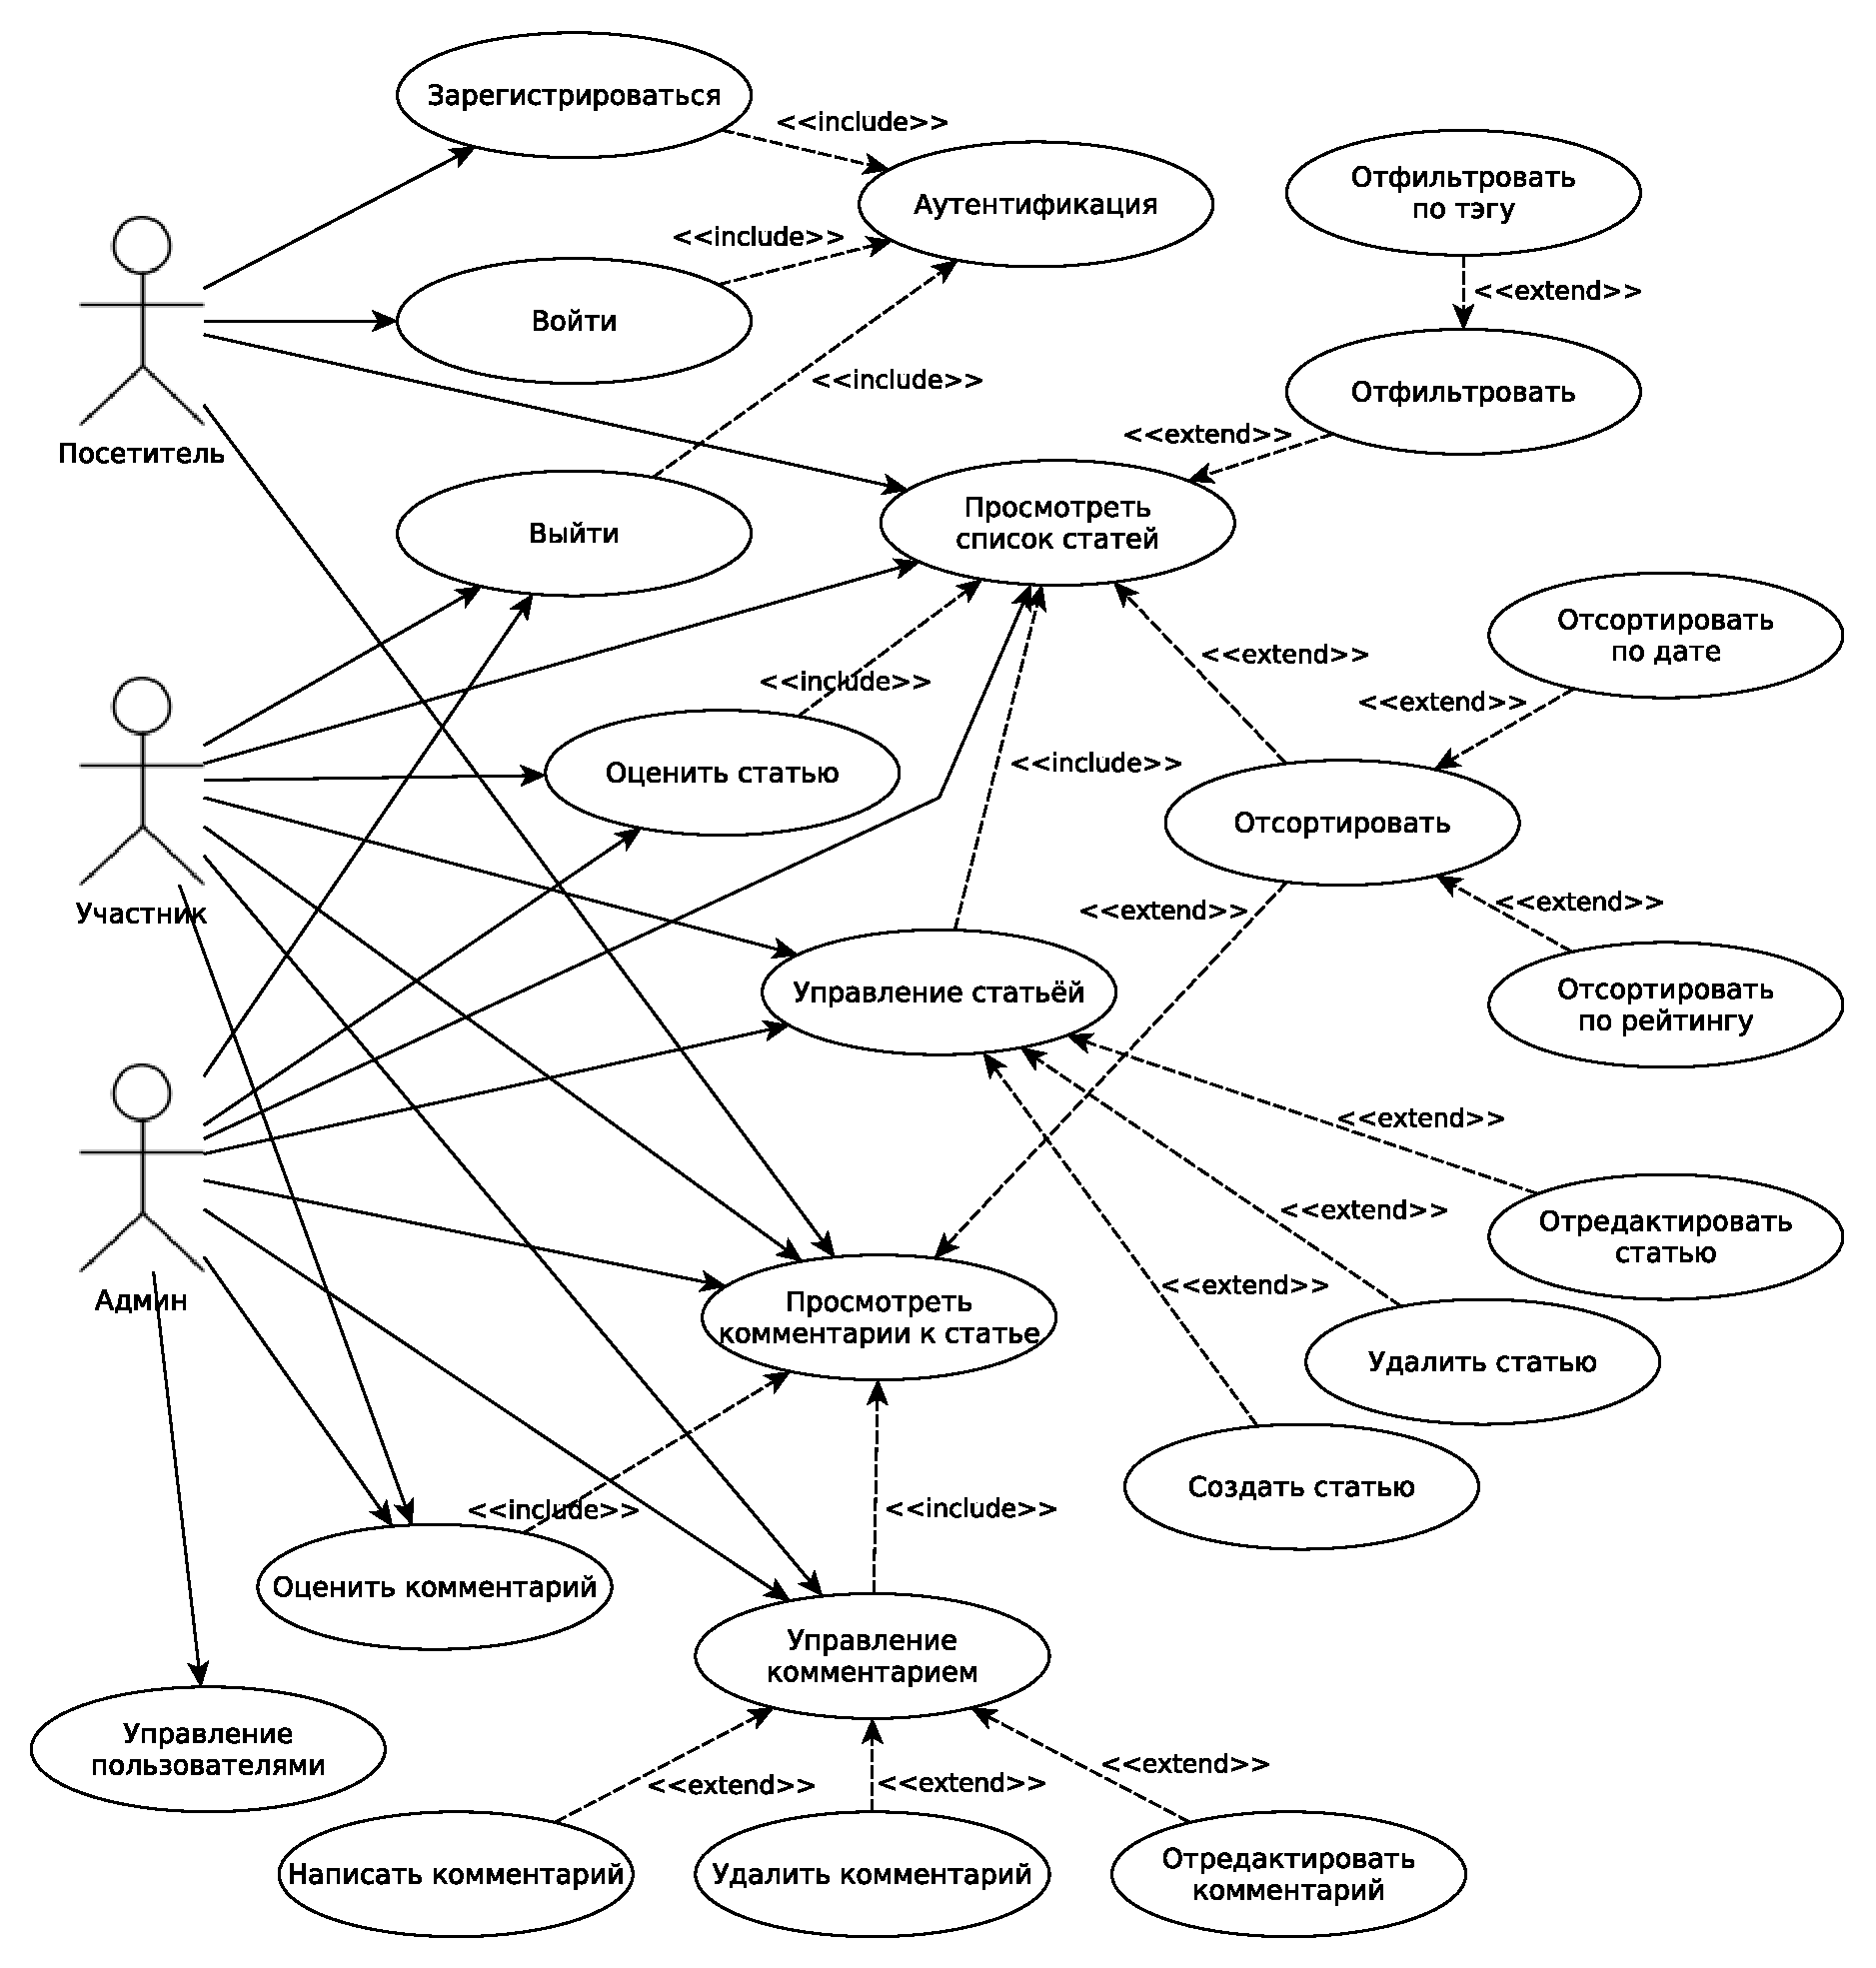
\includegraphics[width=\linewidth]{inc/img/use-case.pdf}
	\caption{Диаграмма вариантов использования}
	\label{img:use-case}
\end{figure}

\section{Диаграмма «сущность — связь»}

На рисунке~\ref{img:er} представлена диаграмма вариантов использования.

\begin{figure}[H]
	\centering
	\includegraphics[width=\linewidth]{inc/img/er}
	\caption{Диаграмма «сущность — связь»}
	\label{img:er}
\end{figure}

\section{Система аутентификации}

Фреймворк Django поставляется с системой аутентификации пользователя.
Она обрабатывает учетные записи пользователей, группы, разрешения и сеансы пользователей на основе файлов cookie \cite{django}.

Система аутентификации Django обрабатывает как аутентификацию, так и авторизацию.
Вкратце, аутентификация подтверждает, что пользователь является тем, кем он себя считает, а авторизация определяет, что разрешено делать аутентифицированному пользователю.
Здесь термин аутентификация используется для обозначения обеих задач.

Наличие встроенной системы аутентификации избавляет от её проектирования.

Система аутентификации состоит из:
\begin{itemize}
	\item пользователей;
	\item разрешений: бинарные флаги, определяющие наличие у пользователя права выполнять определённые действия;
	\item групп: универсальный способ назначения меток и прав на множество пользователей;
	\item настраиваемой системы хеширования паролей;
	\item инструментов для форм и представлений для аутентификации пользователей или для ограничения доступа к контенту;
	\item системы плагинов.
\end{itemize}

Система аутентификации в Django стремится быть очень общей и не предоставляет некоторые функции, обычно встречающиеся в системах веб-аутентификации.
Решения для некоторых из этих распространенных проблем были реализованы в сторонних пакетах:
\begin{itemize}
	\item проверка надежности пароля;
	\item регулирование количества попыток входа;
	\item аутентификация через сторонние сервисы (например, OAuth).
\end{itemize}

\section{Структура базы данных}

В данном разделе будут представлены основные таблицы, выделенные в базе данных.

На рисунке \ref{img:db} представлена схема разрабатываемой базы данных.

\begin{figure}[H]
	\centering
	\includegraphics[width=\linewidth]{inc/img/db}
	\caption{Схема базы данных}
	\label{img:db}
\end{figure}

\subsection{Пользователь}

Описание отношения таблицы пользователей User представлено в~таблице~\ref{tbl:auth_user}.
Стоит заметить, что отдельно создавать таблицу, хранящую информацию о пользователях, не придётся: в системе аутентификации фреймворка Django есть стандартная таблица User, отношение которой содержит все нижеперечисленные атрибуты.

\begin{table}[H]
	\centering
	\caption{Отношение таблицы User}
	\label{tbl:auth_user}
	\begin{tabular}{|l|l|l|}
		\hline
		\textbf{Атрибут} & \textbf{Тип} & \textbf{Описание}          \\ \hline
		id               & int          & Идентификатор пользователя \\ \hline
		username         & varchar(150) & Псевдоним пользователя     \\ \hline
		password         & varchar(128) & Пароль                     \\ \hline
		first\_name      & varchar(30)  & Имя                        \\ \hline
		last\_name       & varchar(150) & Фамилия                    \\ \hline
		email            & varchar(254) & Электронная почта          \\ \hline
		is\_superuser    & boolean      & Является ли админом        \\ \hline
	\end{tabular}
\end{table}

\subsection{Статья}

Описание отношения таблицы статей Article представлено в~таблице~\ref{tbl:myblog_article}.

\begin{table}[H]
	\centering
	\caption{Отношение таблицы Article}
	\label{tbl:myblog_article}
	\begin{tabular}{|l|l|l|}
		\hline
		\textbf{Атрибут} & \textbf{Тип} & \textbf{Описание}       \\ \hline
		id               & int          & Идентификатор статьи    \\ \hline
		user\_id         & int          & Идентификатор автора    \\ \hline
		title            & varchar(80)  & Заголовок               \\ \hline
		body             & text         & Тело статьи             \\ \hline
		pub\_date        & timestamp    & Дата и время публикации \\ \hline
		rating           & int          & Рейтинг статьи          \\ \hline
	\end{tabular}
\end{table}

\subsection{Комментарий}

Описание отношения таблицы комментариев Comment представлено в~таблице~\ref{tbl:myblog_comment}.

\begin{table}[H]
	\centering
	\caption{Отношение таблицы Comment}
	\label{tbl:myblog_comment}
	\begin{tabular}{|l|l|l|}
		\hline
		\textbf{Атрибут} & \textbf{Тип} & \textbf{Описание}                   \\ \hline
		id               & int          & Идентификатор комментария           \\ \hline
		user\_id         & int          & Идентификатор автора комментария    \\ \hline
		article\_id      & int          & Идентификатор комментируемой статьи \\ \hline
		body             & text         & Текст комментария                   \\ \hline
		pub\_date        & timestamp    & Дата и время публикации комментария \\ \hline
		rating           & int          & Рейтинг комментария                 \\ \hline
	\end{tabular}
\end{table}

\subsection{Тэг}

Описание отношения таблицы тэгов Tag представлено в~таблице~\ref{tbl:myblog_tag}.
Для осуществление связи многие ко многим между статьями и тэгами создадим стандартную таблицу article\_tags, отношение которой представлено в таблице \ref{tbl:myblog_article_tags}.

\begin{table}[H]
	\centering
	\caption{Отношение таблицы Tag}
	\label{tbl:myblog_tag}
	\begin{tabular}{|l|l|l|}
		\hline
		\textbf{Атрибут} & \textbf{Тип} & \textbf{Описание}  \\ \hline
		id               & int          & Идентификатор тэга \\ \hline
		tag              & varchar(50)  & Тэг                \\ \hline
	\end{tabular}
\end{table}

\begin{table}[H]
	\centering
	\caption{Отношение таблицы article\_tags}
	\label{tbl:myblog_article_tags}
	\begin{tabular}{|l|l|l|}
		\hline
		\textbf{Атрибут} & \textbf{Тип} & \textbf{Описание}    \\ \hline
		id               & int          & Идентификатор связи  \\ \hline
		article\_id      & itn          & Идентификатор статьи \\ \hline
		tag\_id          & int          & Идентификатор тэга   \\ \hline
	\end{tabular}
\end{table}

\subsection{Голос}

Описание отношения таблицы голосов Vote представлено в~таблице~\ref{tbl:myblog_vote}.
Подразумевается, что проголосовать пользователи могут как за статью, так и за комментарий.
Поэтому, чтобы не создавать две отдельные таблицы голосов, введём атрибут content\_type\_id, меняя значение которого можно голосовать за разный тип контента (статьи, комментария).
Идентификатор object\_id будет ссылаться на запись в таблице с идентификатором типа контента content\_type\_id.
Фреймворк Django по умолчанию индексирует каждую созданную таблицу и добавляет новую запись в таблицу типов контентов, описание отношения которой представлено в таблице \ref{tbl:django_content_type}.

\begin{table}[H]
	\centering
	\caption{Отношение таблицы Vote}
	\label{tbl:myblog_vote}
	\begin{tabular}{|l|l|l|}
		\hline
		\textbf{Атрибут}  & \textbf{Тип} & \textbf{Описание}                           \\ \hline
		id                & int          & Идентификатор голоса                        \\ \hline
		user\_id          & int          & Идентификатор проголосовавшего пользователя \\ \hline
		value             & smallint     & Значение ($+1$ или $-1$)                    \\ \hline
		object\_id        & int          & Идентификатор объекта                       \\ \hline
		content\_type\_id & int          & Идентификатор типа контента                 \\ \hline
	\end{tabular}
\end{table}

\begin{table}[H]
	\centering
	\caption{Отношение таблицы content\_type}
	\label{tbl:django_content_type}
	\begin{tabular}{|l|l|l|}
		\hline
		\textbf{Атрибут} & \textbf{Тип} & \textbf{Описание}           \\ \hline
		id               & int          & Идентификатор типа контента \\ \hline
		app\_label       & verchar(100) & Название приложения         \\ \hline
		model            & verchar(100) & Название модели             \\ \hline
	\end{tabular}
\end{table}

\section{Диаграммы классов}

На рисунках \ref{img:uml-models} и \ref{img:uml-views} представлены UML диаграммы классов моделей и представлений соответственно.

\begin{figure}[H]
	\centering
	\includegraphics[width=\linewidth]{inc/img/uml-models}
	\caption{UML диаграмма классов компонентов доступа данным и бизнес-логики}
	\label{img:uml-models}
\end{figure}

\begin{figure}[H]
	\centering
	\includegraphics[width=\linewidth]{inc/img/uml-views}
	\caption{UML диаграмма классов представлений}
	\label{img:uml-views}
\end{figure}

\section*{Вывод}

Были представлены диаграммы вариантов использования и «сущность~— связь», с помощью которых спроектирована база данных и архитектура приложения, обеспечивающего возможность пользователей авторизовываться и аутентифицироваться, создавать, редактировать и оценивать статьи и комментарии к ним.
